\section*{Ziel}
    In diesem Versuch sollen grundlegende Schaltungen mit Operationsverstärkern aufgebaut und untersucht werden.
    Hierbei sollen Unterschiede zwischen einem realen und idealen Operationsverstärker, sowie einige Anwendungsmöglichkeiten und Grenzen verdeutlicht werden \cite{anleitung}.
\section{Theorie}
    \label{sec:theorie}
    \subsection{Operationsverstärker (OV)}
    Ein Operationsverstärker ist ein elektrisches Bauteil das hauptsächlich auf einem Differenzverstärker basiert.
    \subsection{LM741}
        \begin{figure}[ht]
            \centering
            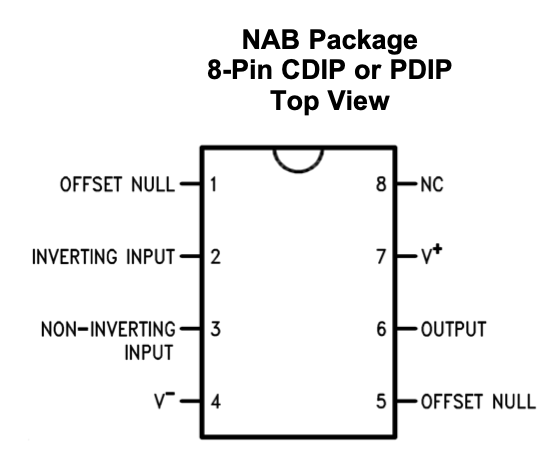
\includegraphics[width = 0.5\textwidth]{bilder/LM741.png}
            \caption{Ein Überblick über die Inputs des Operationsverstärkers LM741}
            \label{fig:LM741}
        \end{figure}
        Der LM741 OV besitzt 8 Kontakte für die verschiedenen Inputs des Verstärkers.
        Um mit dem Verstärker zu arbeiten sind vor allem die zwei Input Kontakte des invertierten Inputs an der Position 2 und des nicht invertierten Inputs an der Position 3 und der Output Kontakt an der Position 6 wichtig.
        Neben diesen Inputs und Outputs für das Verstärken besitzt das Bauteil noch mehrere für den Betrieb notwendige Kontakte.
        Auf Position 1 und 5 befindet sich jeweils ein 'Offset Null' Kontakt.
        Mit Kontakt 4 wird die Betriebsspannung für den invertierten Eingang und mit Kontakt 7 die für den nicht invertierten Eingang geliefert.
        Kontakt 8 ist 'No Connect' (NC) und hat keine Verwendung für den OV.
    \subsection{Invertierender-Linearverstärker}
        Annahme: $U_N = 0$
        Maschenregel:
        \begin{align}
            U_E -U_{R_1}-U_N = 0\\
            U_E -U_{R_1} = 0\\
            U_E = U_{R_1}
        \end{align}
        Knotenregel zwischen $R_1$ und $R_N$:
        \begin{align}
            I_1-I_2 = 0\\
            \frac{U_{R_1}}{R_1} = \frac{U_{R_2}}{R_2}\\
            U_{R_2} = \frac{R_2}{R_1} U_{R_1}\\
            U_{A} = \frac{R_2}{R_1} U_{E}\\
            U_{A} = V' \cdot U_{E}\\
            V' =  \frac{R_2}{R_1} =\frac{U_A}{U_E}
        \end{align}
        
    \subsection{Umkehr-Integrator}
    \subsection{Invertierender-Differenzierer}
    \subsection{nicht-invertierende-Schmitt-Trigger}
    \subsection{Signalgenerator}
    \subsection{Variierende Amplituden}